\documentclass[12pt, twoside]{article}
\usepackage[letterpaper, margin=1in, headsep=0.5in]{geometry}
\usepackage[english]{babel}
\usepackage[utf8]{inputenc}
\usepackage{amsmath}
\usepackage{amsfonts}
\usepackage{amssymb}
\usepackage{tikz}

\usepackage{pgfplots}
\pgfplotsset{width=9cm,compat=1.9}

\usepackage{venndiagram}

\usepackage{graphicx}
\usepackage{enumitem}
\usepackage{multicol}

\usepackage{fancyhdr}
\pagestyle{fancy}
\fancyhf{}
\renewcommand{\headrulewidth}{0pt} % disable the underline of the header

\fancyhead[LE]{\thepage}
\fancyhead[RO]{\thepage \\ Name: \hspace{4cm} \,\\}
\fancyhead[LO]{BECA / Dr. Huson / IB Mathematics\\* Unit 5: Polynomial functions\\* 31 January 2020}

\begin{document}
\begin{enumerate}%[itemsep=0.5cm]
\subsubsection*{5.3 Do Now: Completing the square of quadratic functions}
  \item Let $f$ be a quadratic function. Part of the graph of $f$ is shown below.\\*
  The vertex is at $P(3,-2)$ and the $y$-intercept is at $\displaystyle Q(0, \frac{5}{2})$.\\*
    \begin{center}
    \begin{tikzpicture}
        \foreach \x in {-2, -1,1,2,3,4,5,6}
          \draw[shift={(\x,0)},color=black] (0pt,-3pt) -- (0pt,3pt) node[below]  {$\x$};
        \foreach \y in {-2,-1,1,2,3,4,5,6}
          \draw[shift={(0,\y)},color=black] (2pt,0pt) -- (-2pt,0pt) node[left]  {$\y$};
          \draw [thick, ->] (-2.5,0) -- (+6.5,0) node [right] {$x$};
          \draw [thick, ->] (0,-2.5) -- (0,6.5) node [left] {$y$};
        \fill (3,-2) circle[radius=2pt] node [below] {$P$};
        \fill (0,2.5) circle[radius=2pt] node [right] {$Q$};
        \draw [<->] plot[domain= -1:6] (\x, .5*\x*\x -3*\x +2.5);
    \end{tikzpicture}
    \end{center}
    \begin{enumerate}[itemsep=1cm]
        \item Write down the equation of the axis of symmetry.
        \item The function $f$ can be written in the form $f(x)=a(x-h)^2 +k$. \\*
        Write down the value of $h$ and of $k$.
        \item Find $a$.
        \item Write down the two values of $x$ for which $f(x)=0$.
        \item Hence, write $f$ in factored form, i.e. $f(x)=a(x-x_1)(x-x_2)$
    \end{enumerate}

\newpage
\item Graph the $f(x)=3x^2-12x+7$ on your calculator and use its functions to answer these questions. 
\begin{enumerate}[itemsep=1cm]
    \item Write down the coordinates of the vertex.
    \item Hence or otherwise, express the function in the form $f(x)=3(x-h)^2 +k$.
    \item Solve the equation  $f(x)=0$.
\end{enumerate} \vspace{0.5cm}

\item The diagram below shows part of the graph of the function $f(x)=x^2$.
    \begin{center}
    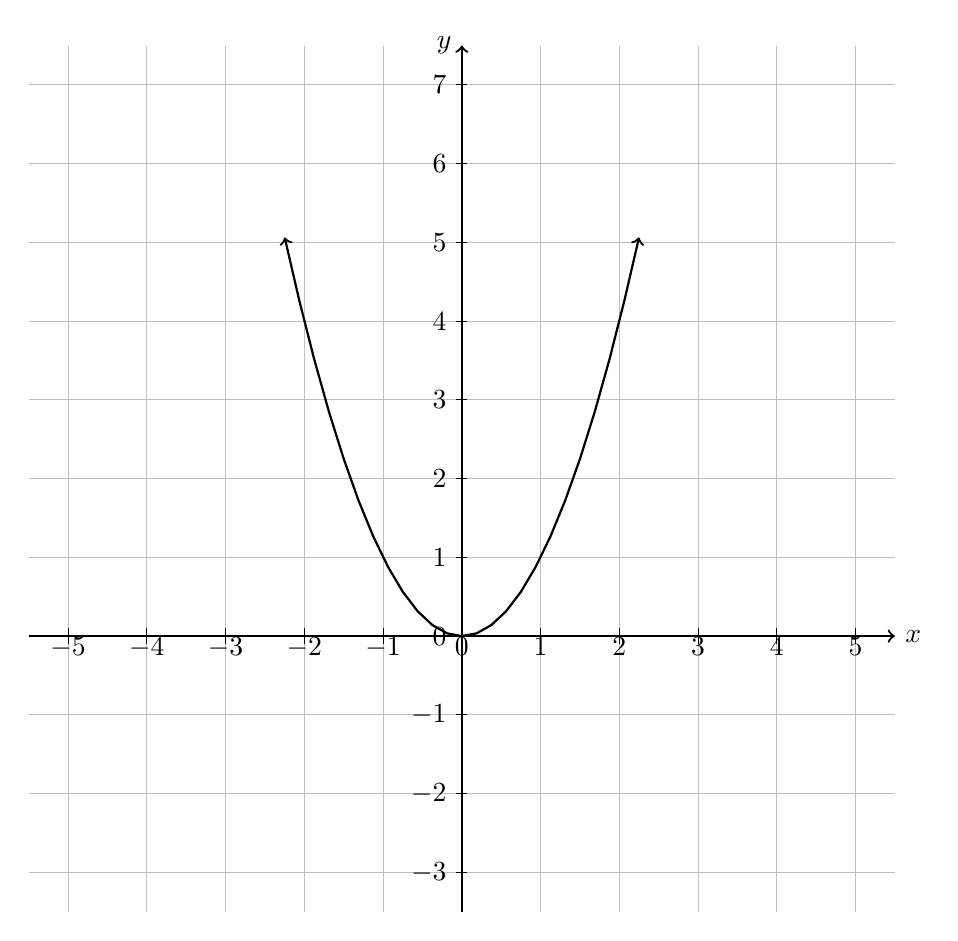
\begin{tikzpicture}
      \draw [thin, color=lightgray,, xstep=1.0cm,ystep=1.0cm] (-5.5,-3.5) grid (5.5,7.5);
      %\draw [thin, color=lightgray,, xstep=0.2cm,ystep=0.2cm] (-5.5,-1.5) grid (5.5,16.5);

      \foreach \x in {-5, -4, -3, -2, -1, 0,1,2,3,4,5}
      \draw[shift={(\x,0)},color=black] (0pt,-3pt) -- (0pt,3pt) node[below]  {$\x$};

      \foreach \y in {-3, -2, -1, 0,1,2,3,4,5, 6,7}
      \draw[shift={(0,\y)},color=black] (2pt,0pt) -- (-2pt,0pt) node[left]  {$\y$};

      \draw [thick, ->] (-5.5,0) -- (+5.5,0) node [right] {$x$};
      \draw [thick, ->] (0,-3.5) -- (0,7.5) node [left] {$y$};

      \draw [thick, <->] plot[domain= -2.25:2.25] (\x, {(\x)*(\x)});

    \end{tikzpicture}
    \end{center}
  \begin{enumerate}
      \item $g(x)$ is the image of $f$ after a translation left 3 and up 2. Draw $g$.
      \item $g$ can be written in the form $g(x)=a(x-h)^2 +k$. Write down $h$ and $k$. \vspace{1cm}
      \item Expand $g$ to standard form, $g(x)=ax^2+bx+c$.
  \end{enumerate}

\newpage
\item Graph the function $f(x)=x^2+2x+2$ over the domain $-1 \leq x\leq 1$.
\begin{itemize}
    \item[(a)] Mark points on the function representing $f(-1)=1$ and $f(1)=5$. Label them as coordinate pairs.
  \item[(b)] Graph and label the inverse of $f$, $f^{-1}(x)$, on the same axes over the domain corresponding to the range of $f$ graphed. Mark the inverses of the points named in part (a), labeling them as coordinate pairs.
  \item[(c)] Write down the domain and range of $f^{-1}(x)$ in the space below. \vspace{2cm}
\end{itemize}
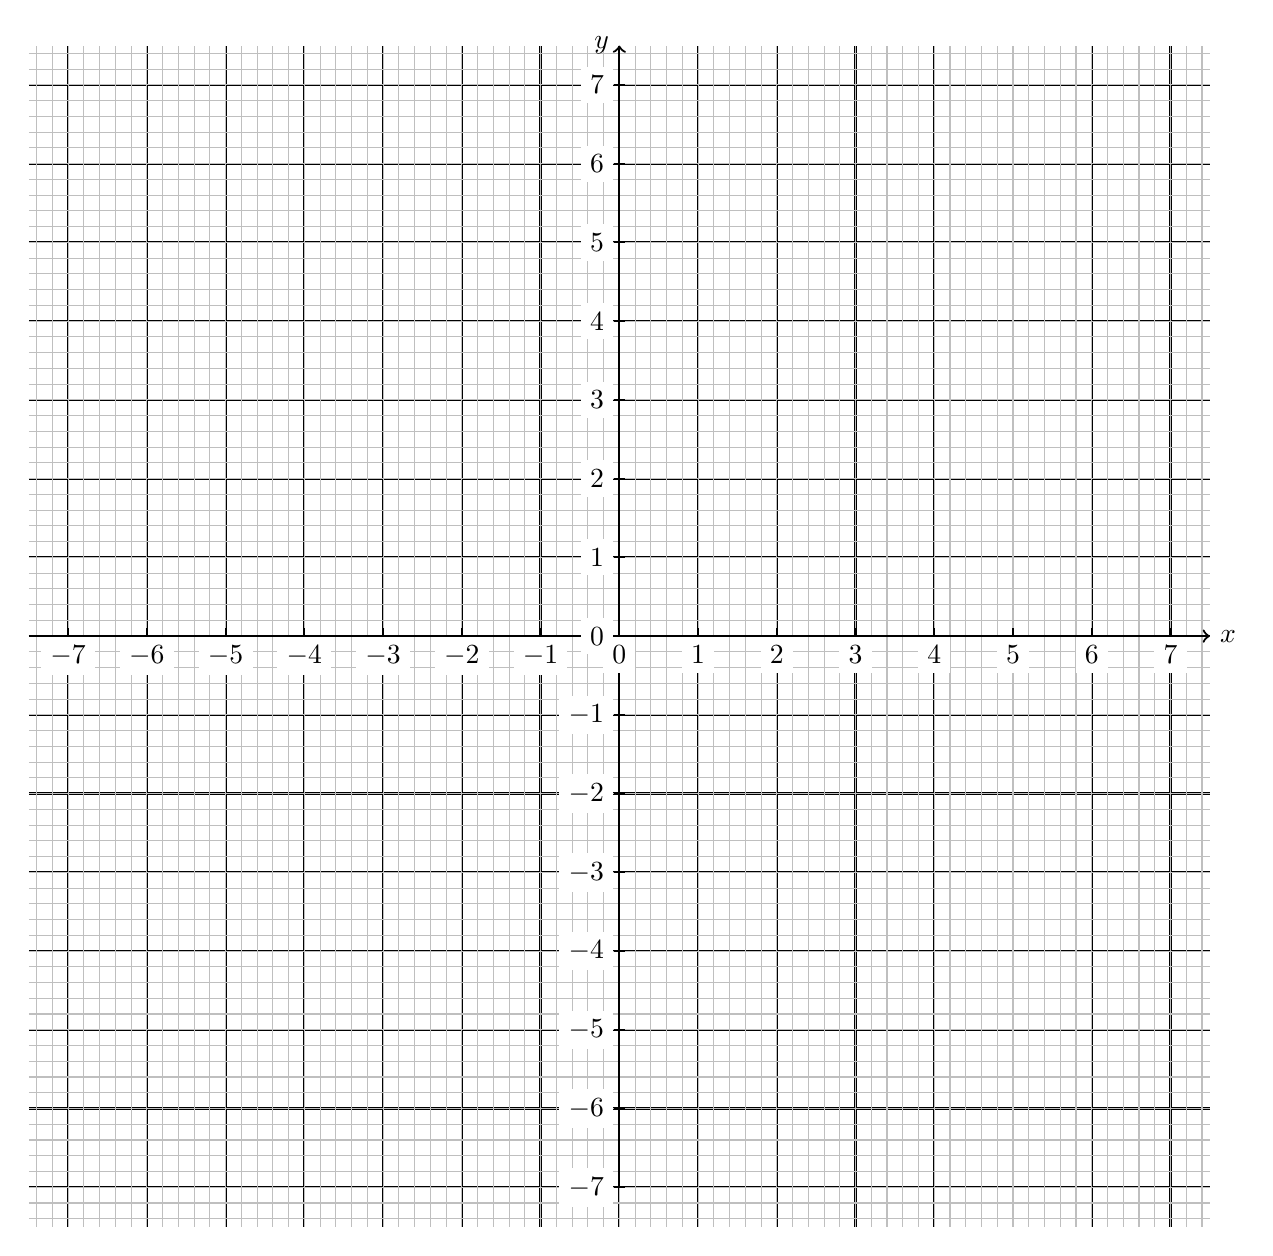
\begin{tikzpicture}[scale=1] %grid with numbered axes, IB cm paper.
  %\clip (-5.5, -1.5) rectangle (5.5, 7.5);
  \draw [thick, color=black,, xstep=1.0cm,ystep=1.0cm] (-7.5,-7.5) grid (7.5,7.5);
  \draw [thin, color=lightgray,, xstep=0.2cm,ystep=0.2cm] (-7.5,-7.5) grid (7.5,7.5);
  \draw [thick, ->] (-7.5,0) -- (+7.5,0) node [right] {$x$};
  \draw [thick, ->] (0,-7.0) -- (0,7.5) node [left] {$y$};
  \foreach \x in {-7,...,7}
    \draw[shift={(\x,0)},color=black] (0pt,-3pt) -- (0pt,3pt) node[below=3pt, fill=white]  {$\x$};
  \foreach \y in {-7,..., 7}
    \draw[shift={(0,\y)},color=black] (2pt,0pt) -- (-2pt,0pt) node[left, fill=white]  {$\y$};

  %\draw [<->, thick] plot[domain= -5:5] (\x, {(3*\x+1)/(\x-2)});
\end{tikzpicture}

\newpage

\item Let $f$ be a quadratic function. Part of the graph of $f$ is shown below.\\*
The vertex is at $P(3,2)$ and the $y$-intercept is at $Q(0, 5)$.\\*

  \begin{center}
    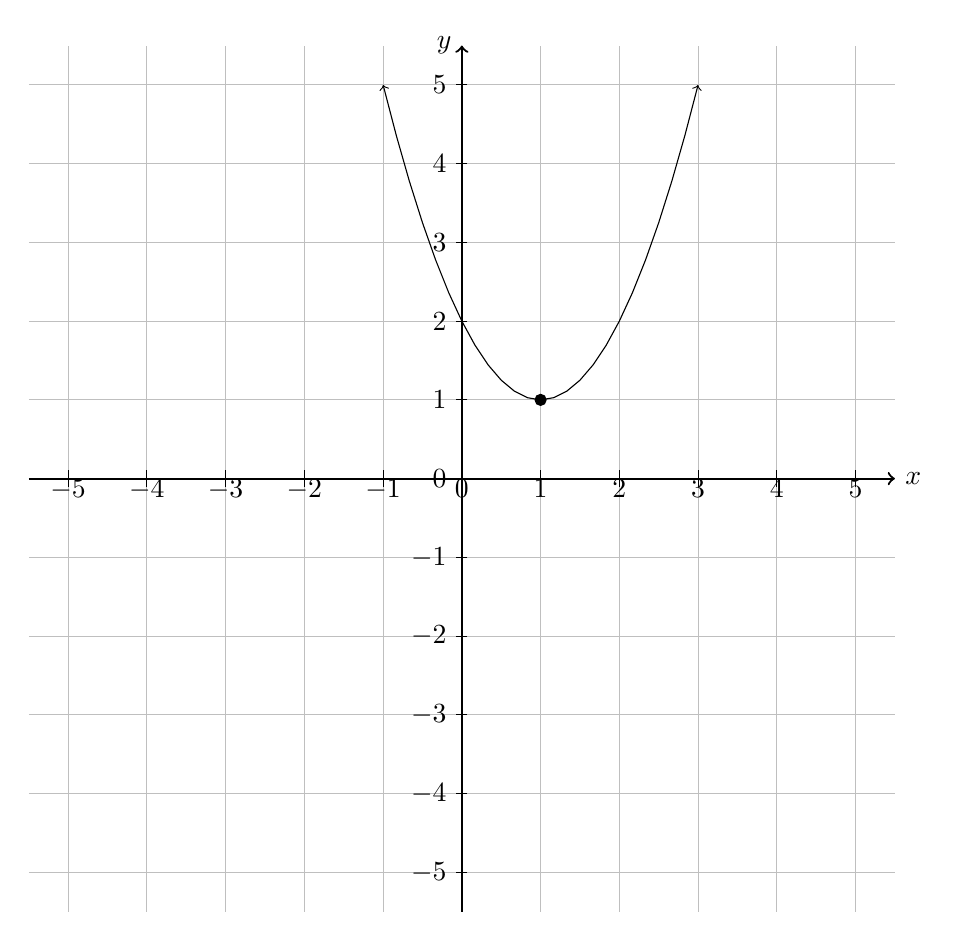
\begin{tikzpicture}
      \draw [thin, color=lightgray,, xstep=1.0cm,ystep=1.0cm] (-5.5,-5.5) grid (5.5,5.5);

      \foreach \x in {-5, -4, -3, -2, -1, 0,1,2,3,4,5}
      \draw[shift={(\x,0)},color=black] (0pt,-3pt) -- (0pt,3pt) node[below]  {$\x$};

      \foreach \y in {-5, -4, -3, -2, -1, 0,1,2,3,4,5}
      \draw[shift={(0,\y)},color=black] (2pt,0pt) -- (-2pt,0pt) node[left]  {$\y$};

      \draw [thick, ->] (-5.5,0) -- (+5.5,0) node [right] {$x$};
      \draw [thick, ->] (0,-5.5) -- (0,5.5) node [left] {$y$};

      \draw (3, 2);
      \draw (1,1) circle[radius=2pt];
      \fill (1,1) circle[radius=2pt];

      \draw [<->] plot[domain= -1:3] (\x, \x*\x -2*\x + 2);  %.5*\x*\x -2*\x +3

    \end{tikzpicture}
  \end{center}
  \begin{enumerate}
      \item Write down the equation of the axis of symmetry.
      \item The function $f$ can be written in the form $f(x)=a(x-h)^2 +k$. \\*
      Write down the value of $h$ and of $k$.
      \item Find $a$.
  \end{enumerate}


\newpage


    \item The following diagram shows the graph of a function $f$.\\
      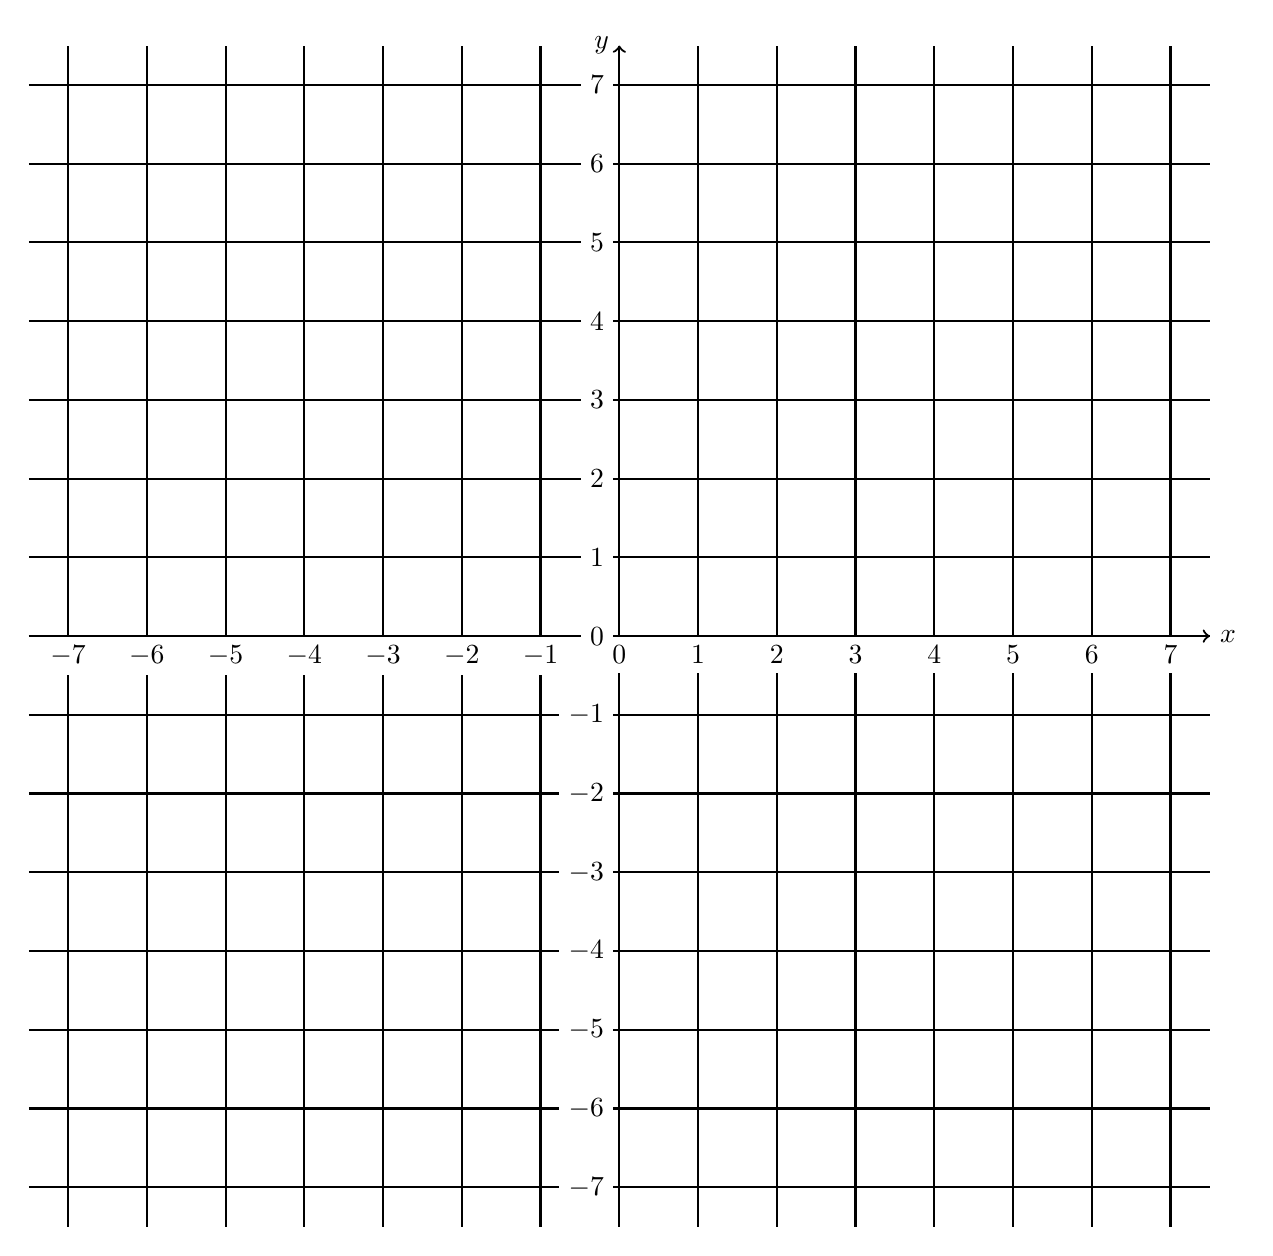
\begin{tikzpicture}[scale=1] %grid with numbered axes, IB cm paper.
        %\clip (-5.5, -1.5) rectangle (5.5, 7.5);
        \draw [thick, color=black,, xstep=1.0cm,ystep=1.0cm] (-7.5,-7.5) grid (7.5,7.5);
        %\draw [thin, color=lightgray,, xstep=0.2cm,ystep=0.2cm] (-7.5,-7.5) grid (7.5,7.5);
        \draw [thick, ->] (-7.5,0) -- (+7.5,0) node [right] {$x$};
        \draw [thick, ->] (0,-7.0) -- (0,7.5) node [left] {$y$};
        \foreach \x in {-7,...,7}
          \draw[shift={(\x,0)},color=black] (0pt,-3pt) -- (0pt,3pt) node[below=3pt, fill=white]  {$\x$};
        \foreach \y in {-7,..., 7}
          \draw[shift={(0,\y)},color=black] (2pt,0pt) -- (-2pt,0pt) node[left, fill=white]  {$\y$};

        %\draw [<->, thick] plot[domain= -5:5] (\x, {(3*\x+1)/(\x-2)});
      \end{tikzpicture}
      \begin{enumerate}
        \item Find $f^{-1}(x)$.
        \item Find $(f \circ f)(-1)$.
        \item On the same diagram, sketch the graph of $y=-f(x)$.
      \end{enumerate}

    \item The following diagram shows part of the graph of a quadratic function $f$.

\newpage

    \newpage
    Graphing calculators may be used on this section.

    \item Let $f(x)=2x^2+3x-1$.
    \begin{enumerate}
        \item Write down the coordinates of the vertex.
        \item Hence or otherwise, express the function in the form $f(x)=2(x-h)^2 +k$.
        \item Solve the equation  $f(x)=0$.
    \end{enumerate}

    \item Consider the function $f(x)=x^2-6x-1$.
    \begin{enumerate}
        \item Sketch the graph of $f$, for $-4 \leq x \leq 3$.
        \item This function can also be written in the form $f(x)=(x-p)^2 -10$.\\*
        Write down the value of $p$.
        \item The graph of $g$ is obtained by reflecting the graph of $f$ in the $x$-axis, followed by a translation of $(0, 4)$.\\* Show that $g(x)=x^2+3x-1$.
        \item The graphs of $f$ and $g$ intersect at two points.\\*
        Write down the x-coordinates of these two points.
    \end{enumerate}

\newpage


    %missing: identifying a function vs relation,


\item Consider the equation $x^2 + (k-2)x=-4$, where $k$ is a real number. Find the values of $k$ for which the equation has two equal real solutions.


  \end{enumerate}
\end{document}
